\chapter{Georeferencing}
\section{Georeferencing with point cloud}

It is possible to set session as ground truth.
Thus, optimization process (Pose GRAPH SLAM) will not change its poses.
Other sessions can be aligned against ground truth session by adding edges.

\begin{figure}[H]
	\centering
	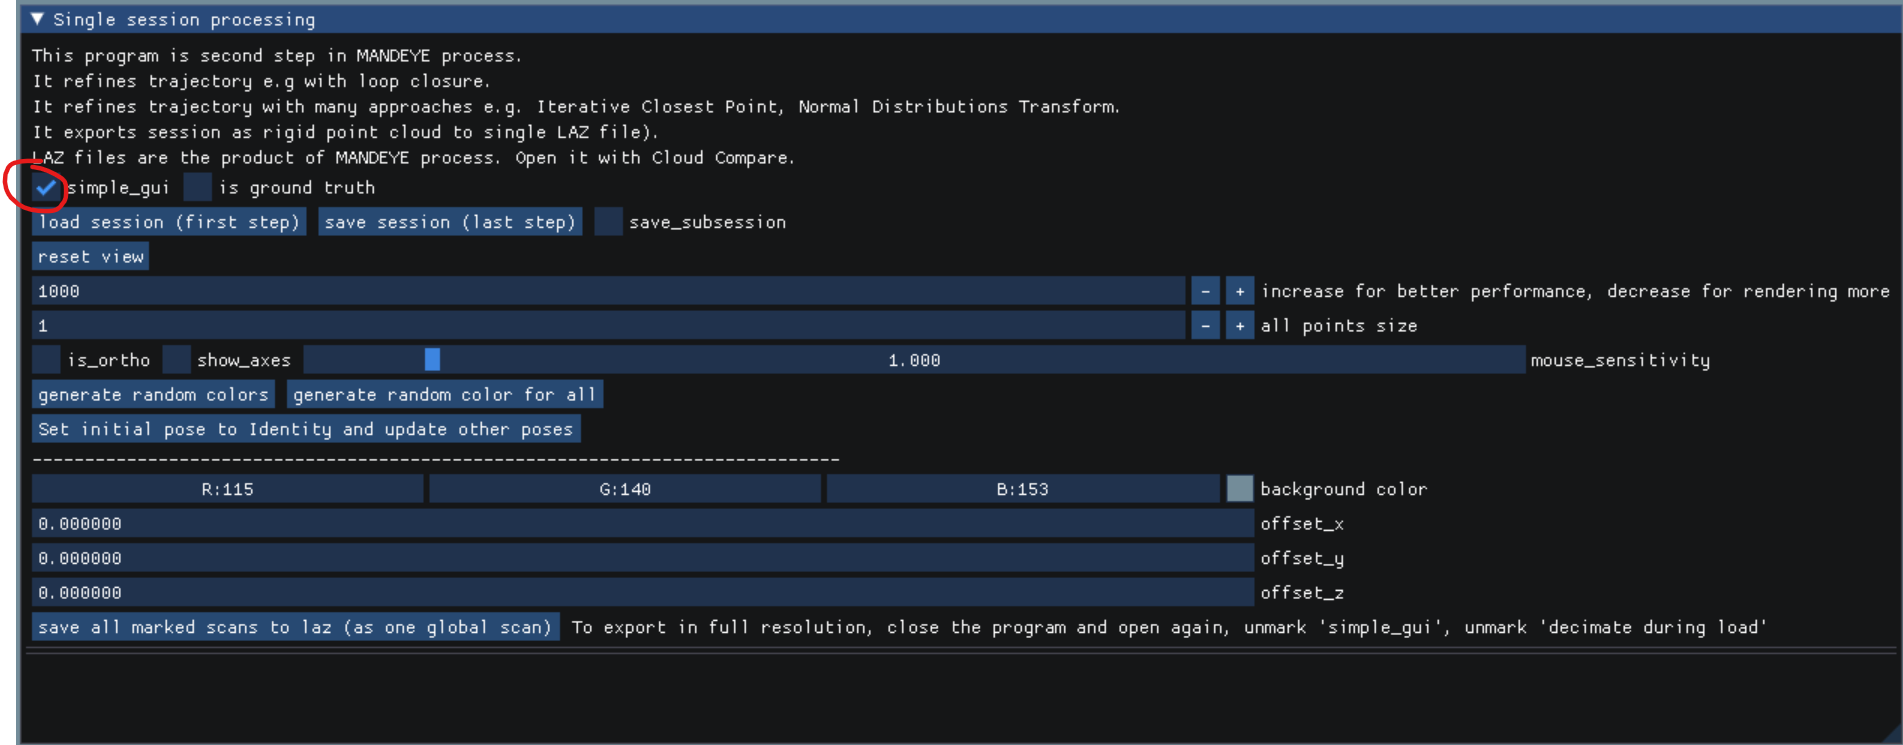
\includegraphics[width=\textwidth]{g1.png}
	\caption{Use multi view tls registration step2 program to open TLS files.}
	\label{fig:g1}
\end{figure}

\begin{figure}[H]
	\centering
	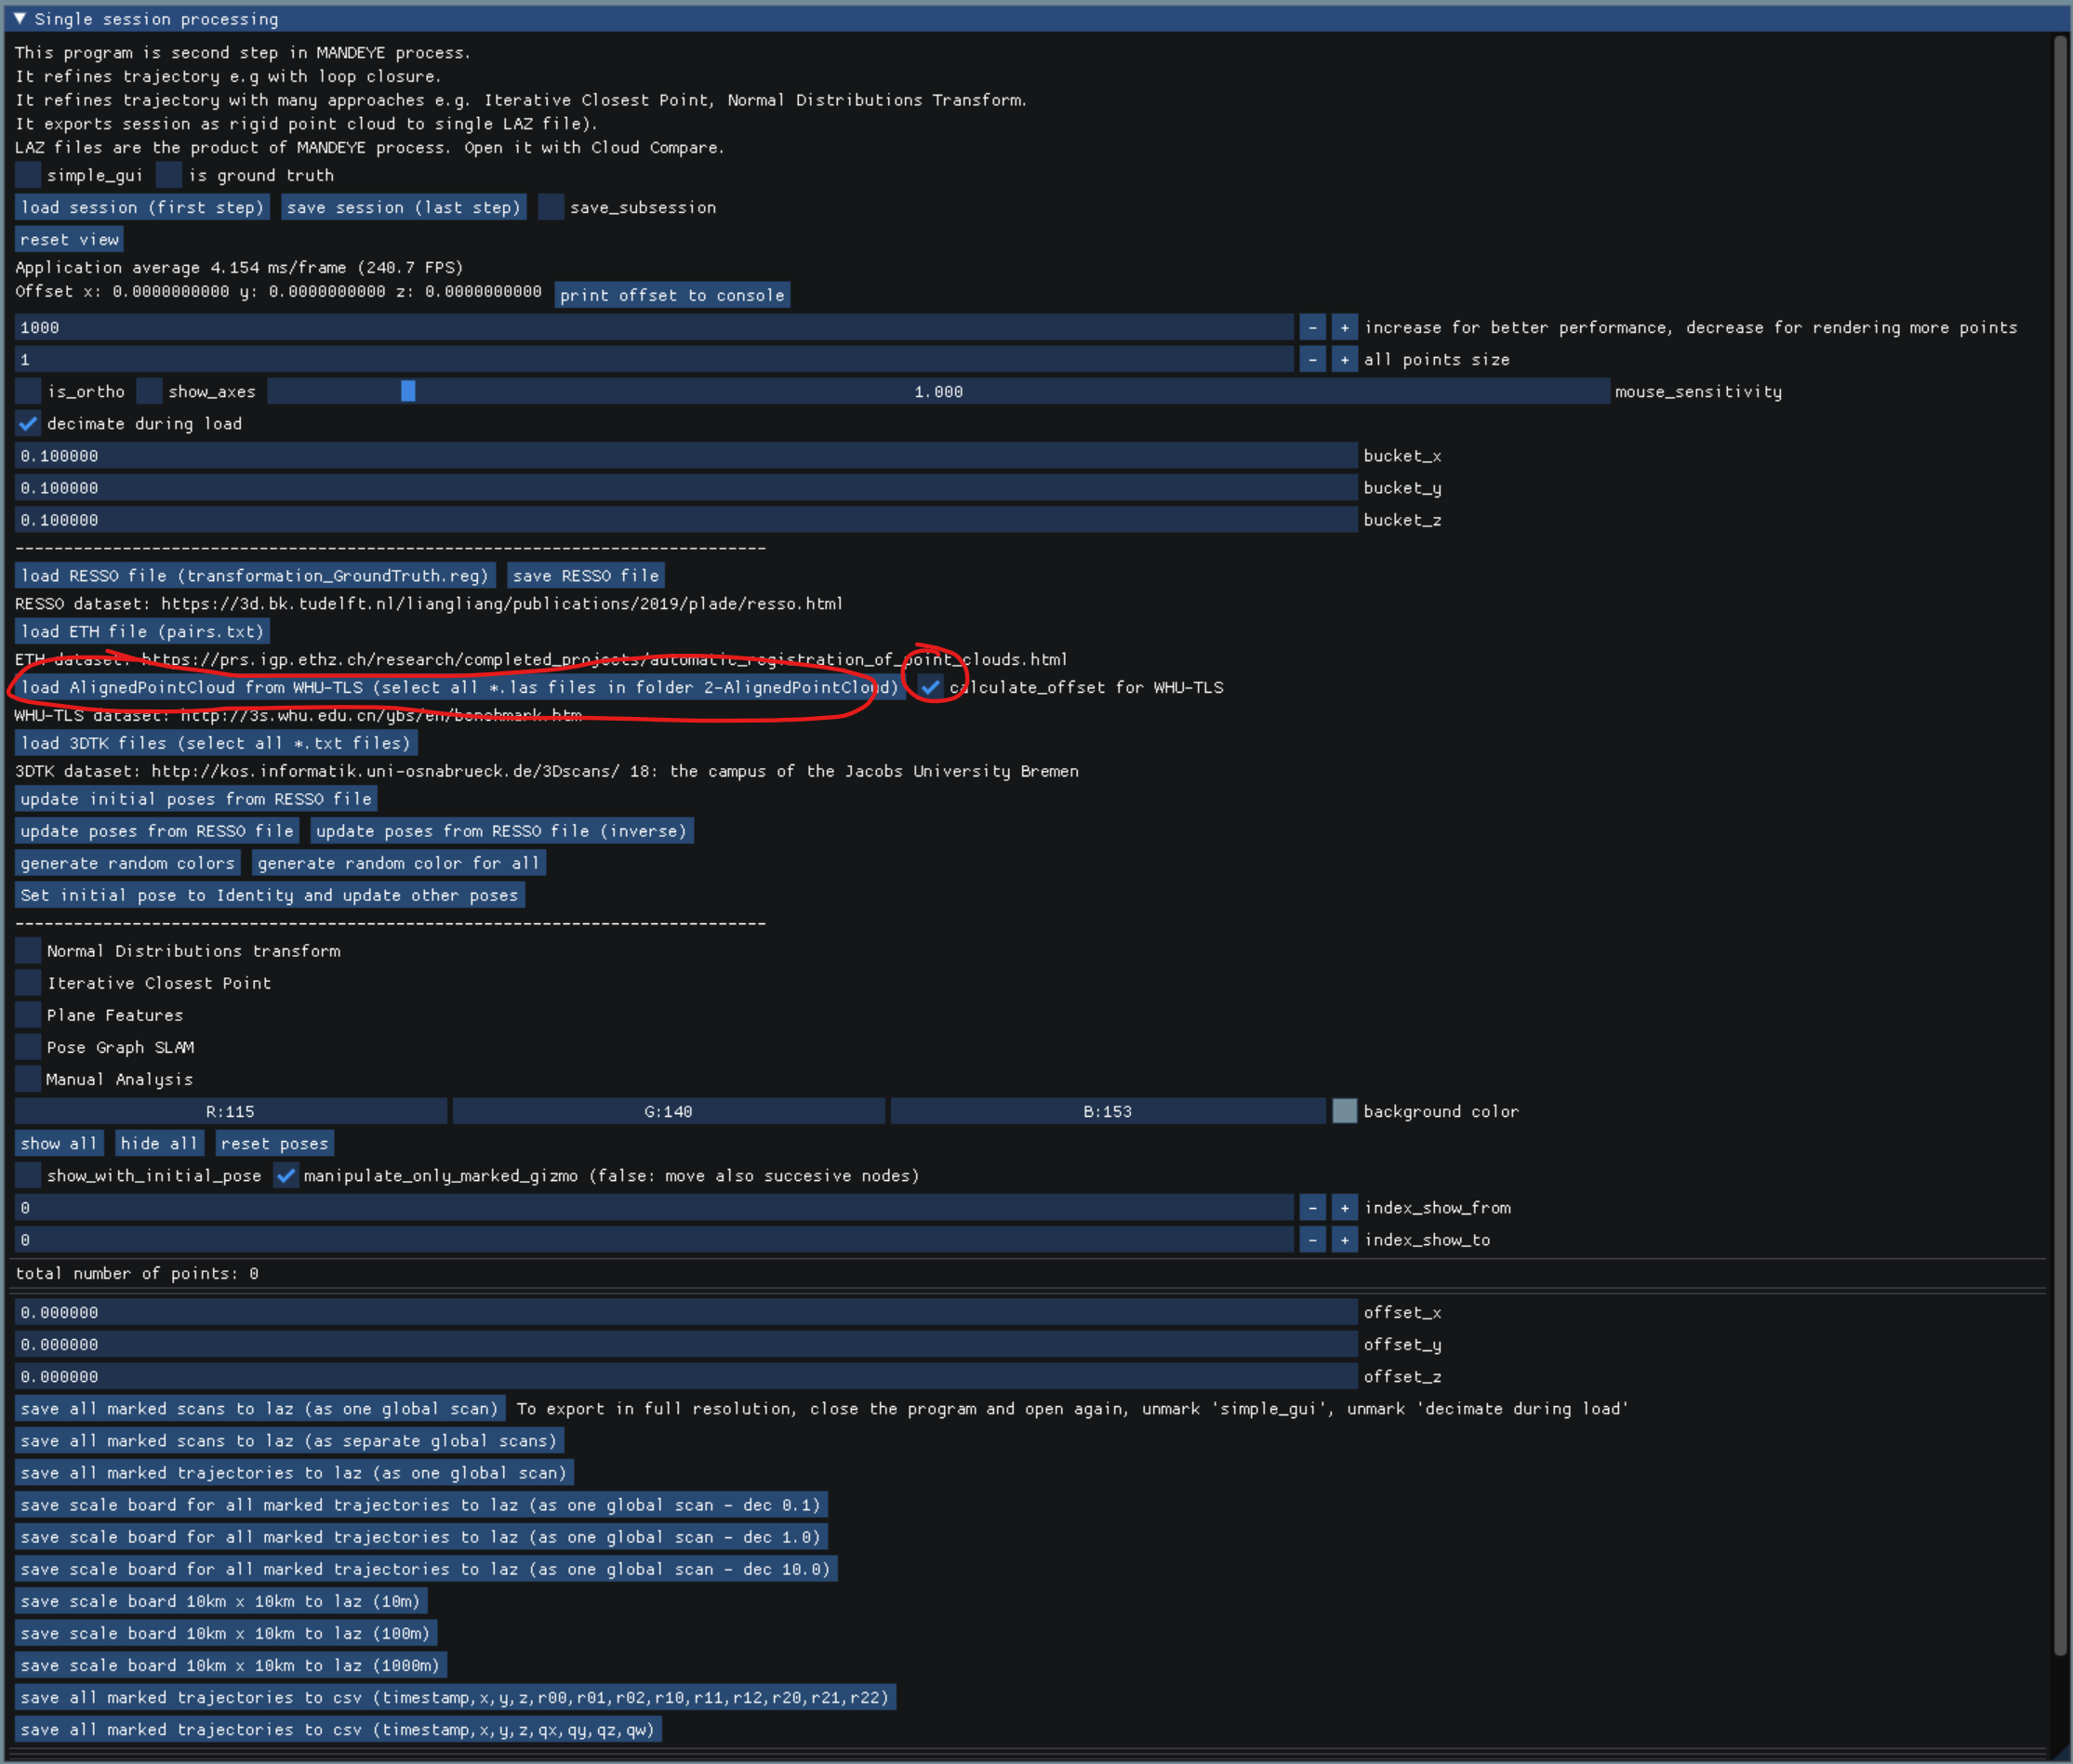
\includegraphics[width=\textwidth]{g2.png}
	\caption{Mark calculate offset for WHU-TLS, load AlignedPointCloud from WHU-TLS (select all *.las/laz files in folder)}
	\label{fig:g2}
\end{figure}

\begin{figure}[H]
	\centering
	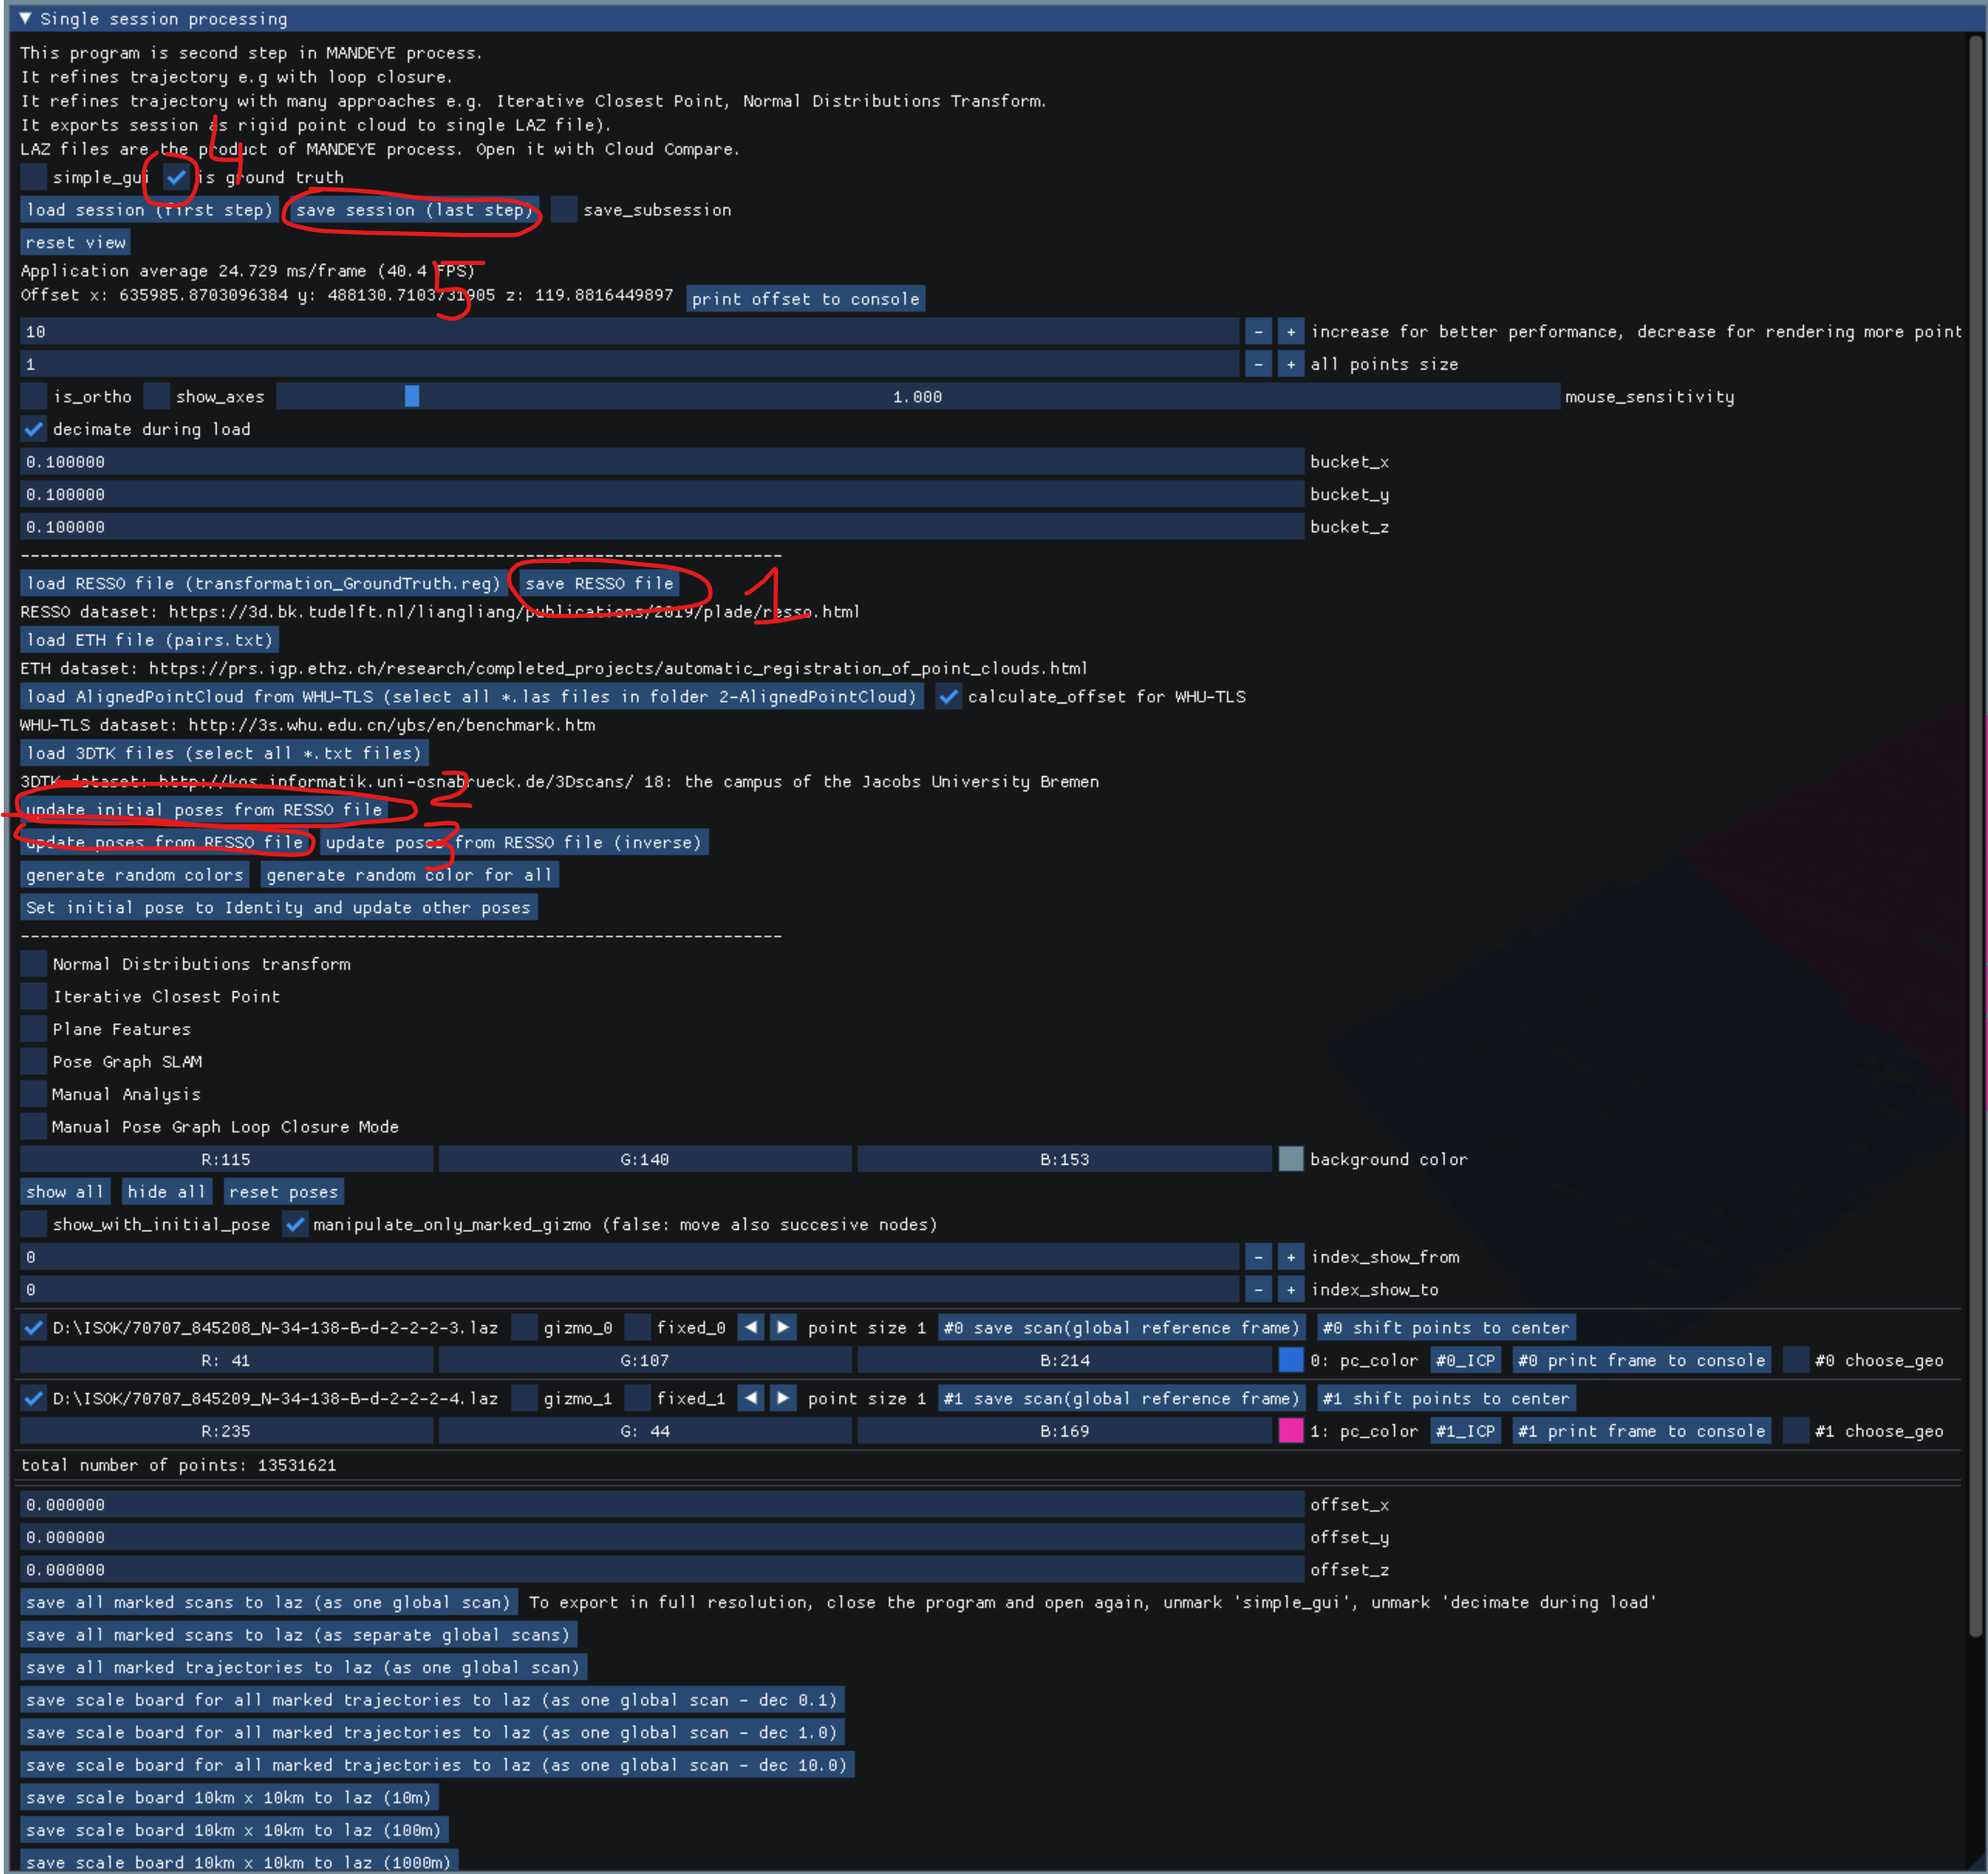
\includegraphics[width=\textwidth]{g3.png}
	\caption{1: save RESSO file, 2: update initial poses from RESSO file (select file from 1), 3: update poses from RESSO file (select file from 1), 4: set checkbox is ground truth, 5: save session.}
	\label{fig:g3}
\end{figure}

\section{Georeferencing with WGS84toCartesian}
\label{Georeferencing_with_WGS84toCartesian}
It uses \url{https://github.com/chrberger/WGS84toCartesian/tree/master} WGS84toCartesian.
It is a small and efficient library written in modern C++ library to convert WGS84 latitude/longitude positions to/from Cartesian positions using Mercator projection.
If You have MANDEYE with GNSS receiver, then it saves data in gnssXXXX.gnss files.
This is ASCII file with\\
---\\
timestamp lat lon alt hdop satelites-tracked height age time fix-quality\\
---\
\begin{figure}[H]
	\centering
	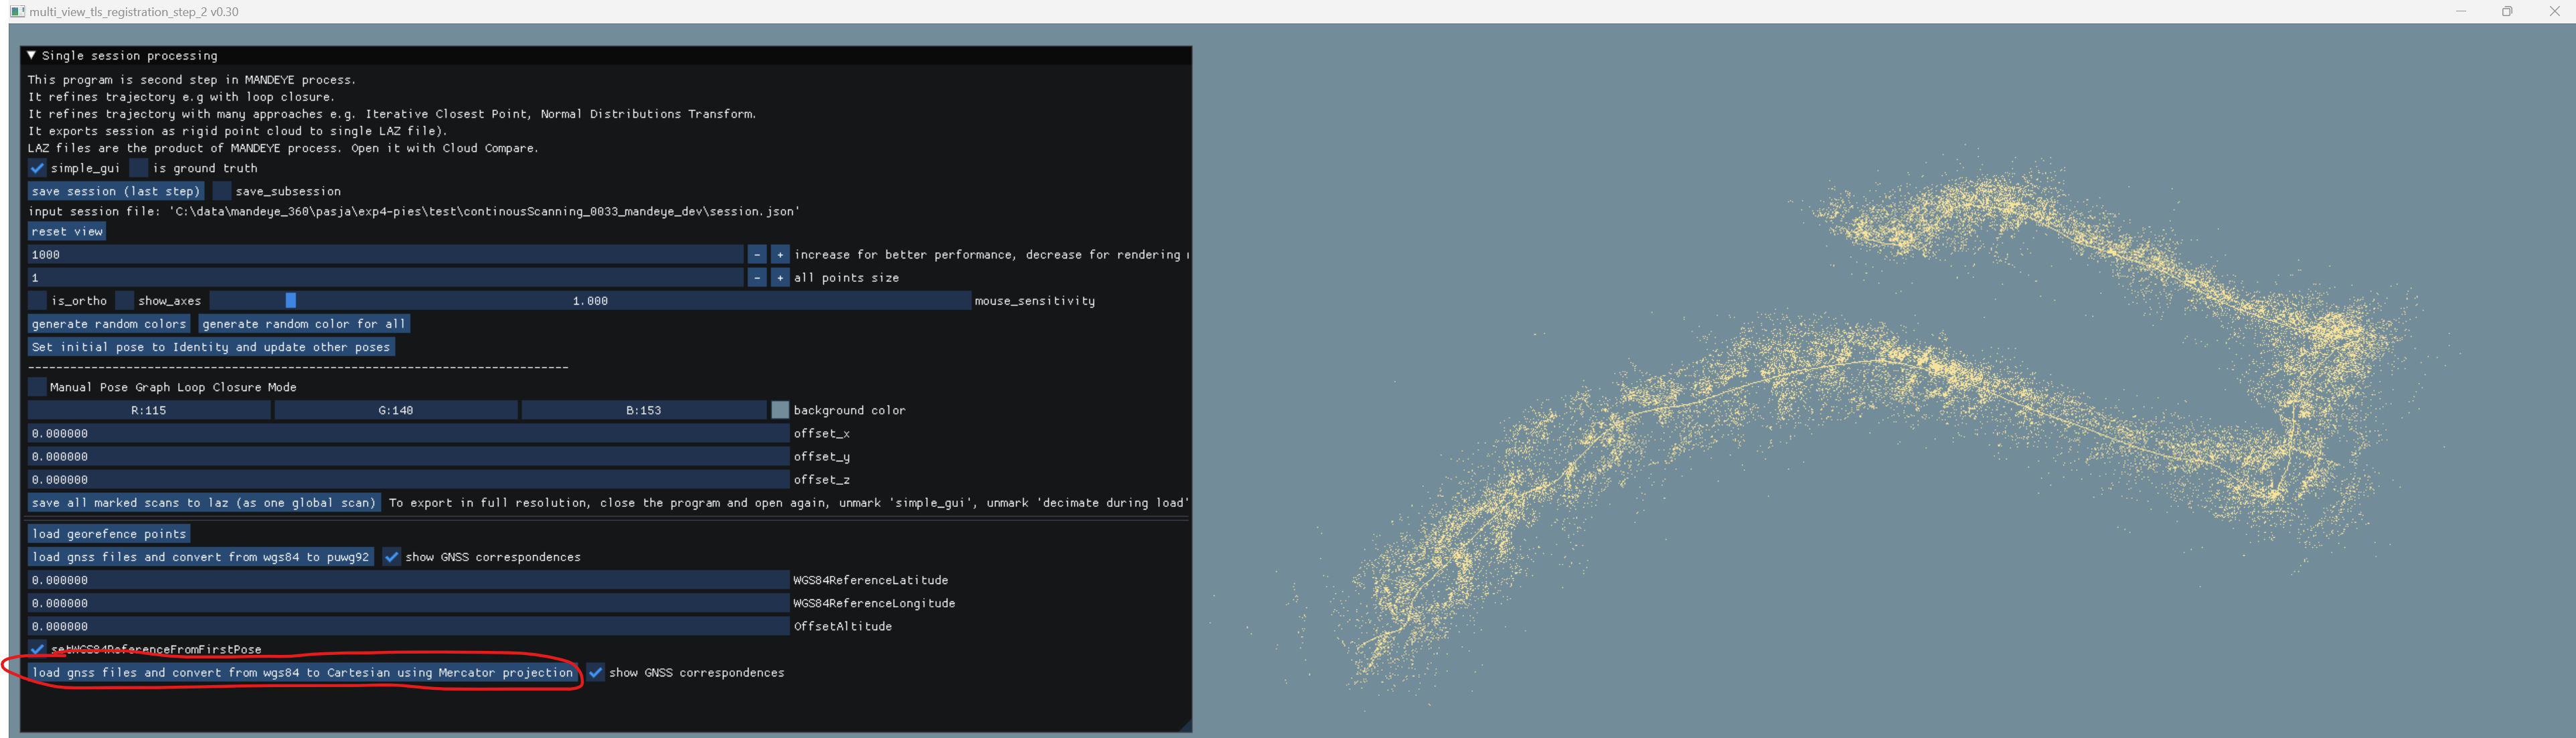
\includegraphics[width=\textwidth]{geo0.png}
	\caption{Georeferencing step 1: load gnss files and convert from wgs84 to Cartesian using Mercator projection.}
	\label{fig:geo0}
\end{figure}

\begin{figure}[H]
	\centering
	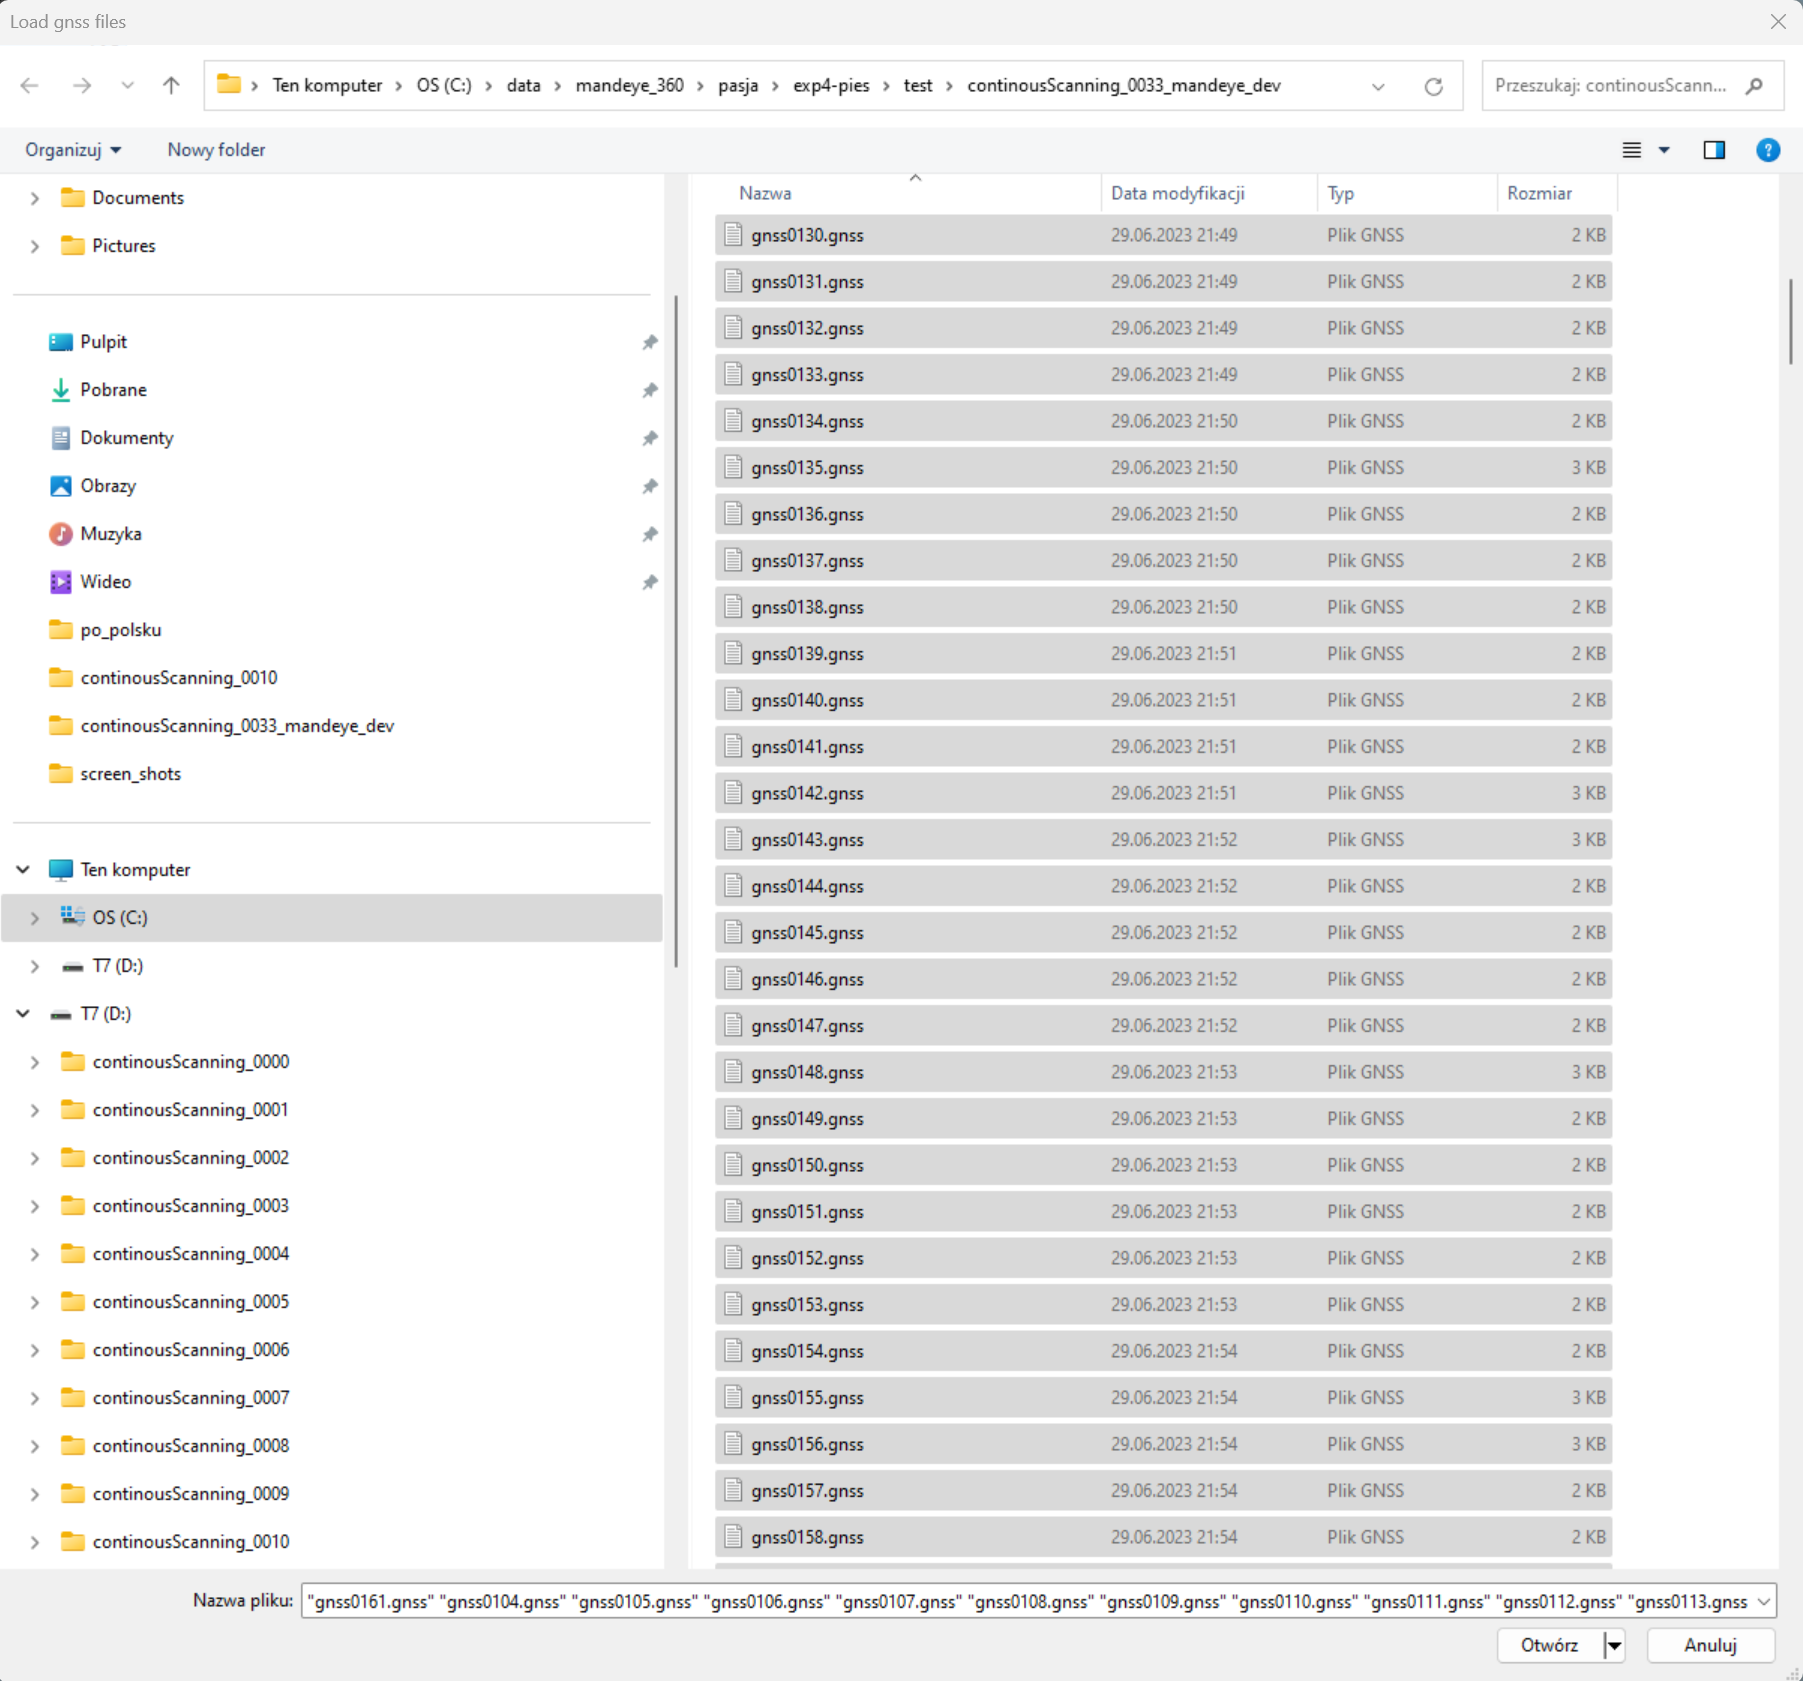
\includegraphics[width=\textwidth]{geo1.png}
	\caption{Georeferencing step 2: mark all gnss files and load.}
	\label{fig:geo1}
\end{figure}

\begin{figure}[H]
	\centering
	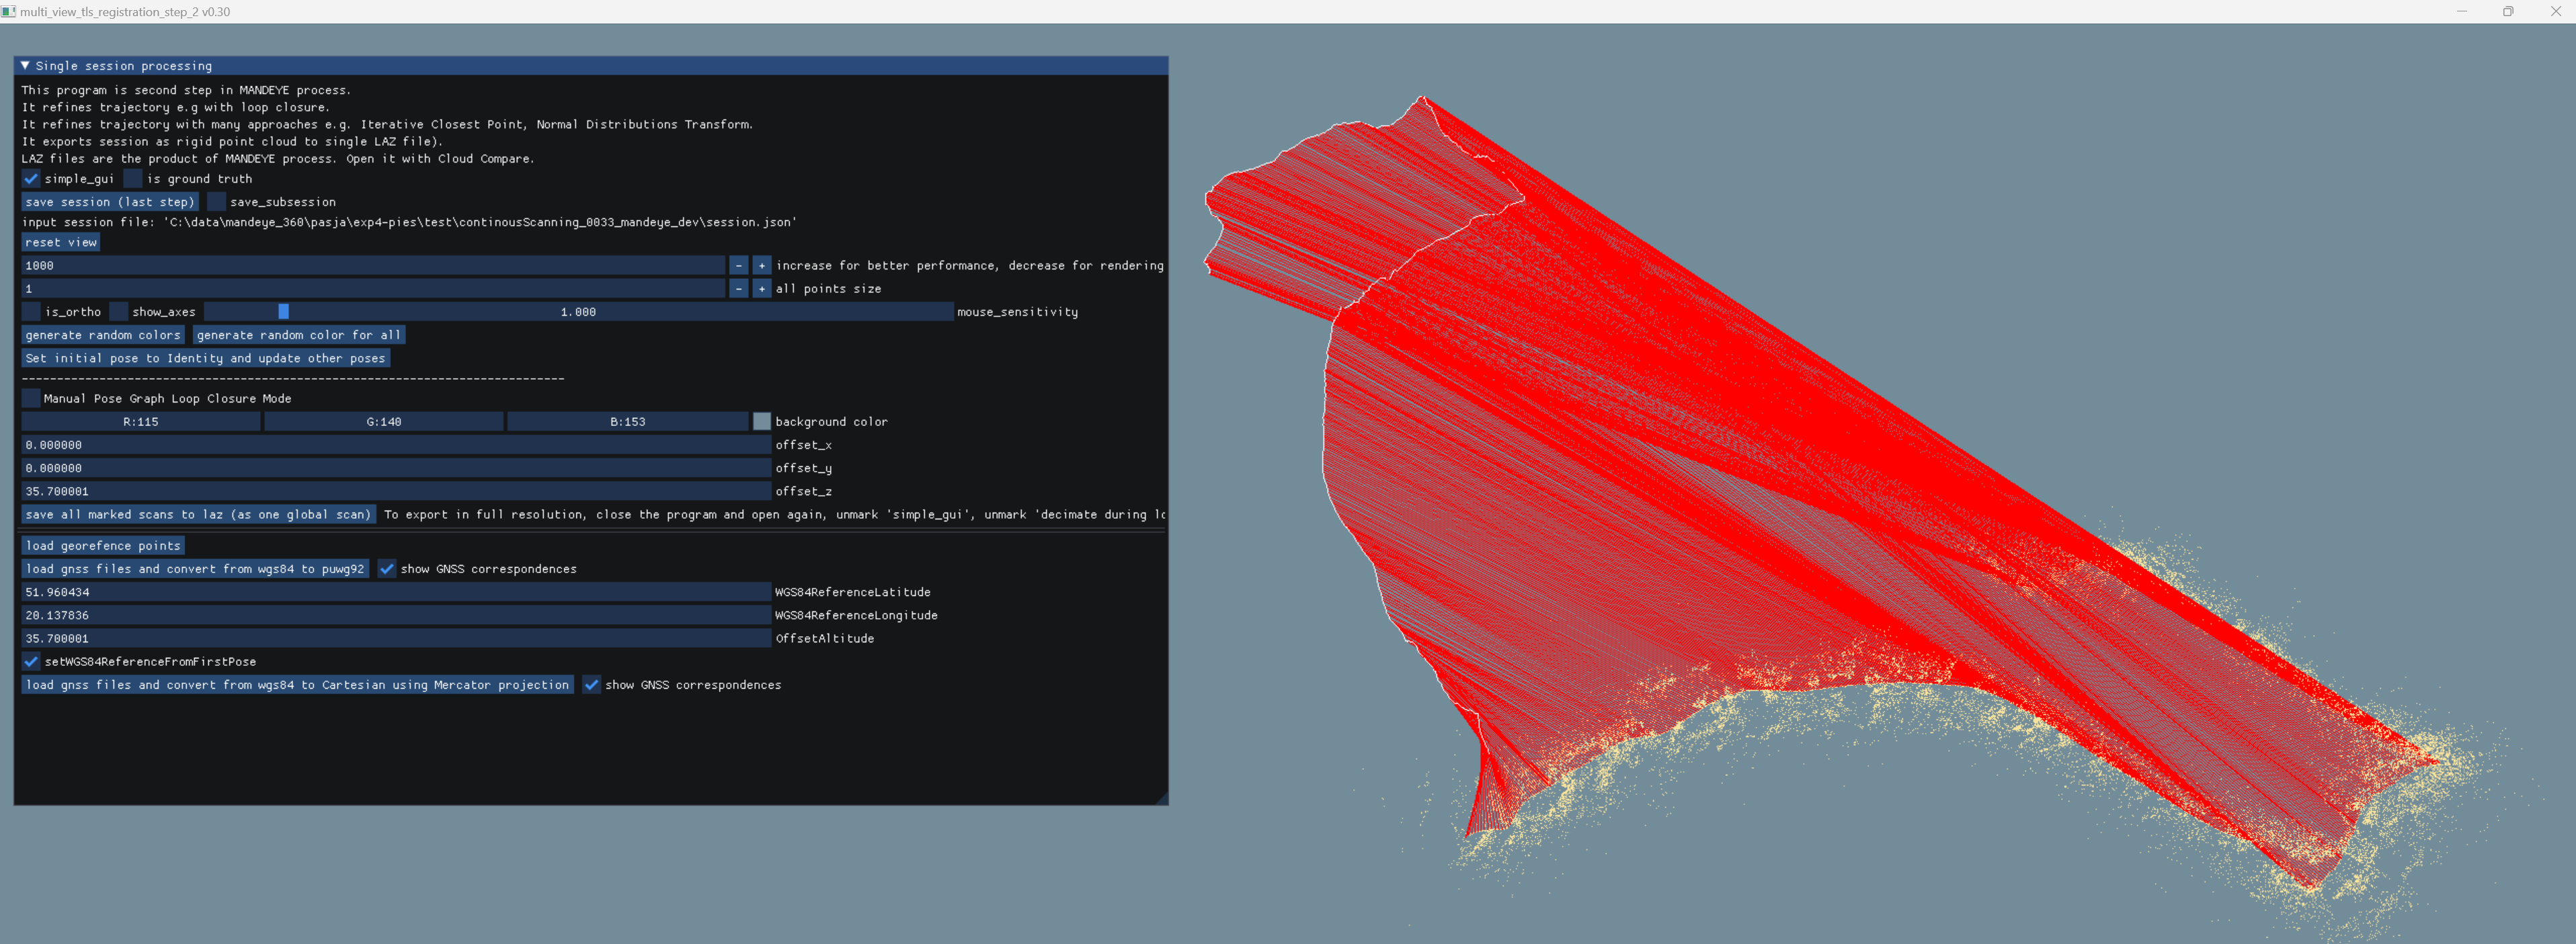
\includegraphics[width=\textwidth]{geo2.png}
	\caption{Georeferencing step 3: check/uncheck 'show GNSS correspondences' to see gnss-poses correspondences. Remark: You can use gizmo for manual initial trajectory to GNSS alignment.}
	\label{fig:geo2}
\end{figure}

\begin{figure}[H]
	\centering
	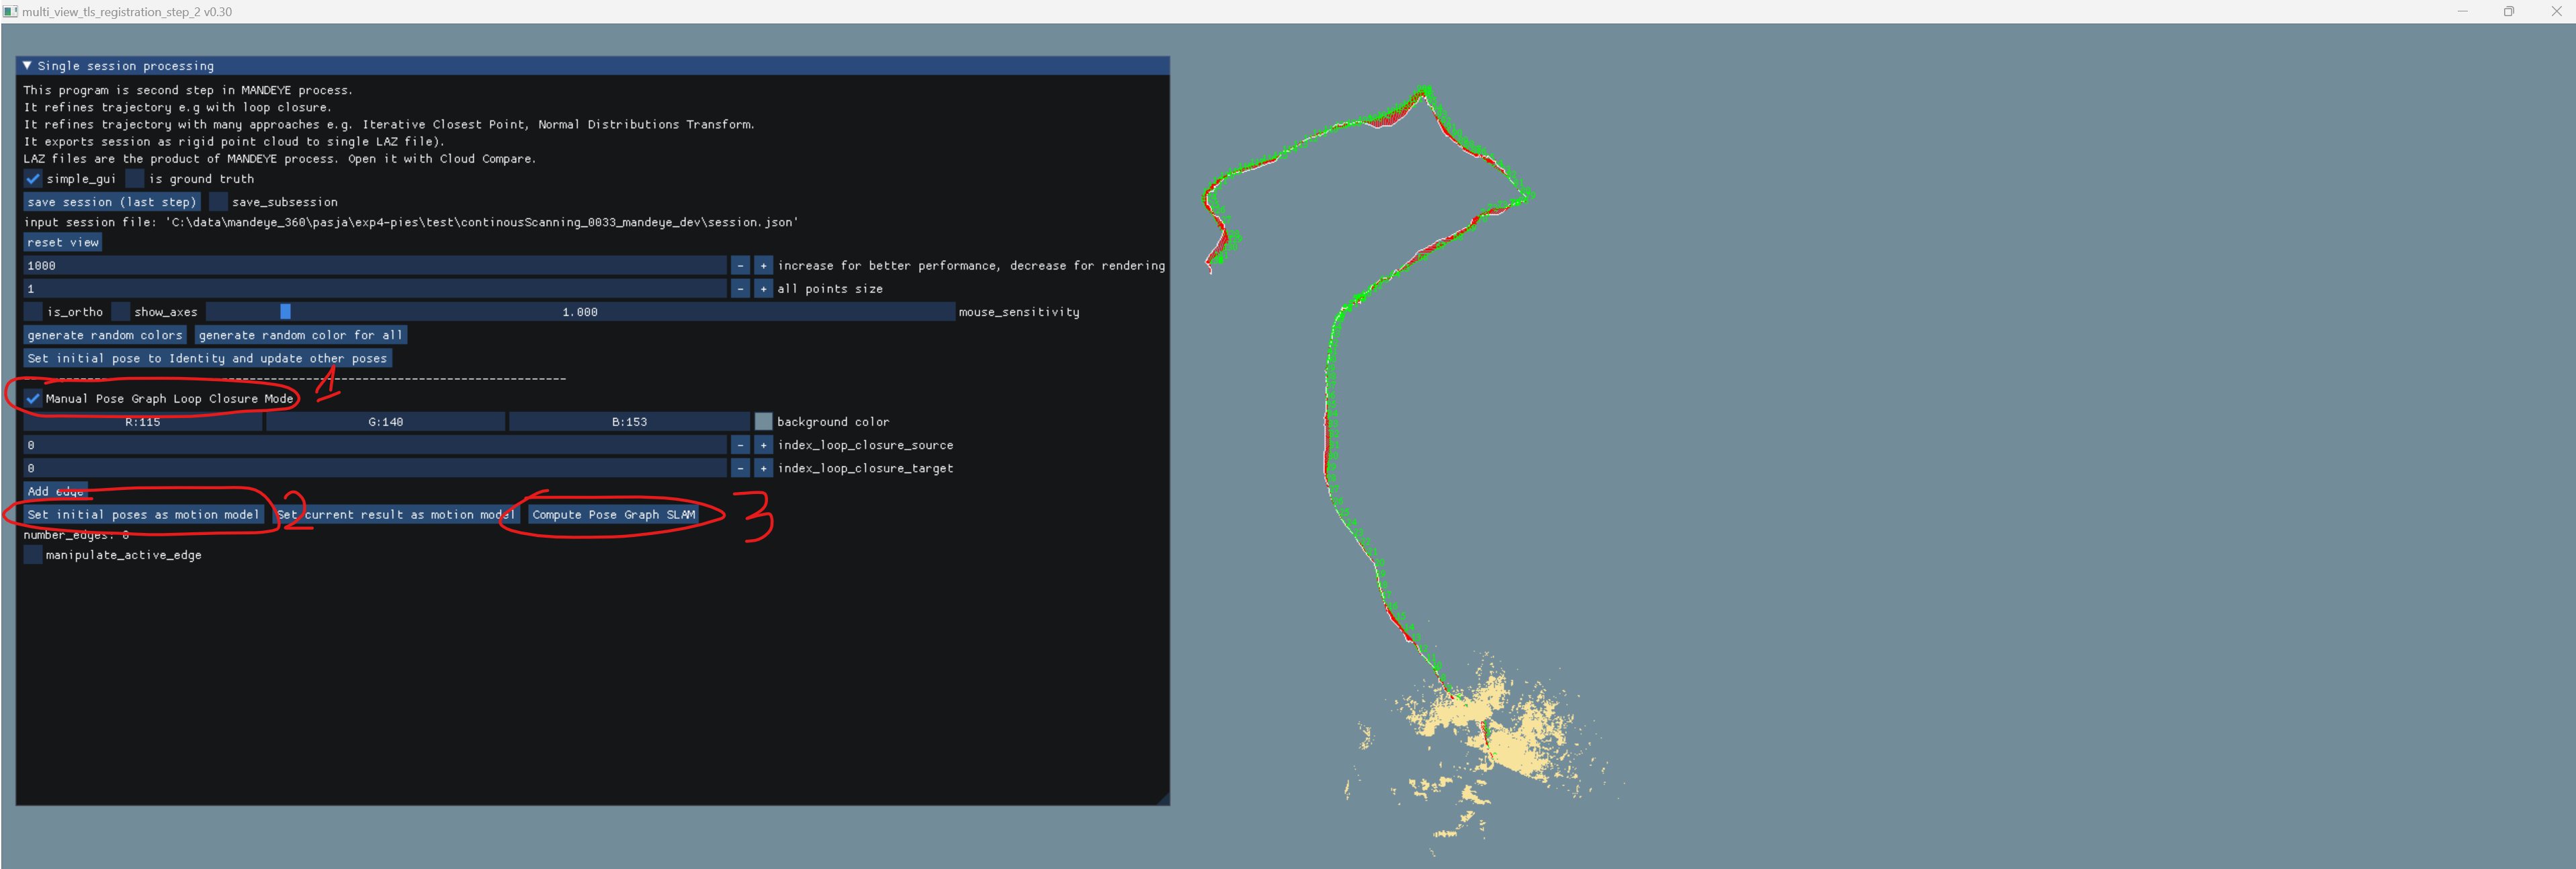
\includegraphics[width=\textwidth]{geo3.png}
	\caption{Georeferencing step 4: Check Manual Pose Graph Loop Closure Mode, then set initial poses as motion model, then Compute Pose Graph SLAM.}
	\label{fig:geo3}
\end{figure}